\documentclass[a4paper, UTF8]{ctexart}				%中文环境
%\documentclass{article}							%英文环境

%---------------------------宏包加载----------------------------
    \usepackage{amsmath}
    \usepackage{amssymb}
    \usepackage{amsthm}
    \usepackage{geometry}
        \geometry{left = 2.54cm, right = 2.54cm,
            top = 3.18cm, bottom = 3.18cm}			%页边距设置
    \usepackage{fancyhdr}
        \pagestyle{fancy}
        %\lfoot{\today}   							%左页脚
        \cfoot{\thepage}							%中页脚
        %\rfoot{林陈冉}	 						 		%右页脚
        \setlength{\parskip}{0.5 \baselineskip}		%段距
    \usepackage{hyperref}  							%打开超链接
        \hypersetup{colorlinks=false}				%取消超链接颜色
    \usepackage{tikz}
    \usepackage{multirow}

%---------------------------标题设置----------------------------
    \title{并行程序设计第2次作业}
    \author{林陈冉}
    \date{\today}

%---------------------------定理环境----------------------------
    \newtheorem{theo}{\bf 定理}[section]			  %新建定理环境, 标题为"定理", 以section为计数器标记
    \newtheorem{define}{\bf 定义}[section]
    \newtheorem{algo}{\bf 算法}
    \renewcommand{\proofname}{\bf 证明}			  %重命名定理环境, 标题为"证明"
    \numberwithin{equation}{section}				%以section为计数器标记公式

%-----------------------------正文------------------------------
\begin{document}									%开始正文
    \maketitle										%生成标题
    \paragraph{分析}
        设 $x = \{x_1, x_2, \cdots, x_n\}, y = \{y_1, y_2, \cdots, y_n\} \in \mathbb{R}^n$ , $x$ 和 $y$ 的内积为 
        \[
            \langle{x},{y}\rangle  = \sum^{n}_{k = 1} x_k y_k
        \]
        需要执行 $n$ 次乘法和 $n - 1$ 次加法.
        
        这个过程中数据彼此依赖度很小, 改成并行计算时, 设有 $p$ 个处理器, 可以把 $x$ , $y$ 拆成 $p$ 个向量, 求出内积后再求和, 即 
        \begin{equation*}
            \begin{split}
                x^i = \{x_{f(i)}, x_{f(i) + 1}, \cdots, x_{f(i+1)-1}\}, \quad 
                &y^i = \{y_{f(i)}, y_{f(i) + 1}, \cdots, y_{f(i+1)-1}\}, \quad
                i \in \{1, 2, \cdots, p\}\\
                \langle{x},{y}\rangle = &
                \sum^{p}_{i=1} \langle{x^i},{y^i}\rangle = 
                \sum^{p}_{i=1} \sum^{f(i+1)-1}_{k=f(i)} x_k y_k
            \end{split}
        \end{equation*}
        其中 $f$ 是一个映射, 它把 $\{1, 2, \cdots, n\}$ 给分成 $p$ 份. 考虑到各处理器运算能力接近, 可以简单进行等分, 即
        $$
            f(i) = \begin{cases}
                (i - 1) \lceil \frac{n}{p} \rceil &, i=1, 2, \cdots, p\\
                n &, i = p + 1
            \end{cases} 
        $$

    \paragraph{计算}
        串行程序运行用时 
        \[
            T_1 = n + n-1 = 2n - 1
        \]
        当有 $p$ 个处理器 
        \[
            T_p = 2 \lceil \frac{n}{p} \rceil - 1 + \log_2 p
        \]
        那么加速比为 
        \[
            S_p = \frac{T_1}{T_p} = \frac{2n - 1}{2 \lceil \frac{n}{p} \rceil - 1 + \log_2 p}
        \]
        效率 
        \[
            E_p = \frac{S_p}{p} = \frac{2n - 1}{2p \lceil \frac{n}{p} \rceil - p + p\log_2 p}
        \]

        现在我们想保证效率为定值 $E$ , 记 $K = \frac{E}{1 - E}$
        $$
                T_0 - \frac{T_1}{K} = 0 
                \quad \Rightarrow \quad
                F(p) = 2p \lceil \frac{n}{p} \rceil - p + p\log_2 p - (1 + K)(2n - 1) = 0
        $$
        这个方程并不容易解, 先考虑 $p \lceil \frac{n}{p} \rceil$
        \[
            n \le p \lceil \frac{n}{p} \rceil < n + p
        \]
        那么可以得到估计 $F_{up}(p) = -p + p\log_2 p + 1 - (1 + K)(2n - 1)$ , $F_{down}(p) = p + p\log_2 p + 1  - (1 + K)(2n - 1)$ , 且有关系
        \[
            F_{up}(p) \le F(p) < F_{down}(p)
        \]

        \begin{figure}[h]\small\centering
            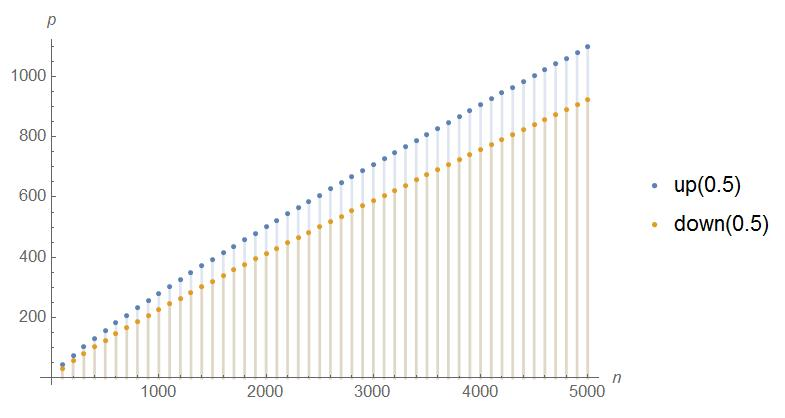
\includegraphics[width=12cm]{1.jpg}\caption{固定效率0.5时$n-p$关系图}\label{fig:1}
        \end{figure}
        
        容易证明, 函数 $F_{up}(p)$ , $F_{down}(p)$ 都是递减的. 那么令它们等于 $0$ 就可以给出 $p$ 的上下界. 图\ref{fig:1}即固定效率 $E_p = 0.5$ 时的估计, 散点曲线 $up(0.5)$ 是 $F_{up}(p) = 0$ 的解, 散点曲线 $down(0.5)$ 是 $F_{down}(p) = 0$ 的解. 可以看出, 存在明显的线性关系.

        \begin{figure}[h]\small\centering
            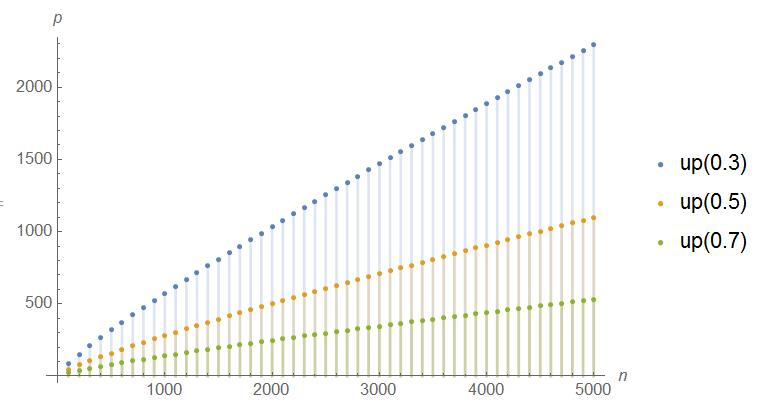
\includegraphics[width=12cm]{2.jpg}\caption{不同效率时$n-p$关系图}\label{fig:2}
        \end{figure}

        图\ref{fig:2}显示了不同效率下的表现, 都取 $p$ 的上估计(以下各图都是如此), 即  $F_{up}(p) = 0$ 的解, 散点曲线 $up(0.3)$ 表示效率 $E_p = 0.3$ 时的处理器个数 , 其他曲线同理. 可以看出, 若想保证效率, 需要用更少的处理器.\newpage

        \begin{figure}[h]\small\centering
            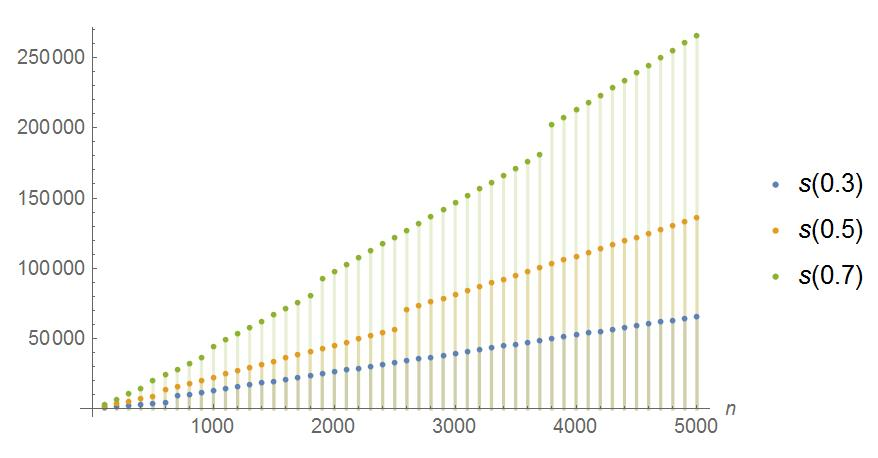
\includegraphics[width=12cm]{3.jpg}\caption{不同效率时$n-S_p$关系图}\label{fig:3}
        \end{figure}

        图\ref{fig:3}显示了不同效率下的加速比, 散点曲线 $s(0.3)$ 表示效率 $E_p = 0.3$ 时的加速比 , 其他曲线同理. 可以看出, 保证效率少用处理器后, 计算速度变慢.

        \begin{figure}[h]\small\centering
            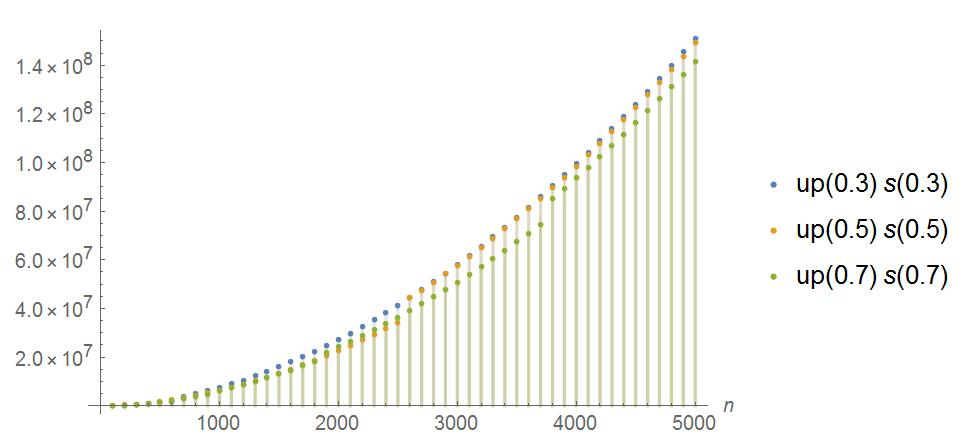
\includegraphics[width=12cm]{4.jpg}\caption{不同效率时$n-p\times S_p$关系图}\label{fig:4}
        \end{figure}

        图\ref{fig:4}显示了不同效率下的加速比与处理器个数的乘积, 散点曲线 $up(0.3)s(0.3)$ 表示效率 $E_p = 0.3$ 时的加速比与处理器个数的乘积 , 其他曲线同理. 可以看出, 无论保证效率为多少, 加速比与处理器个数的乘积是不变的.
\end{document}										%结束正文
